\documentclass{article}
\usepackage{graphicx} % Required for inserting images
\usepackage[
    backend=biber,
    style=phys,
    autocite=superscript % This tells \autocite to behave as a superscript
]{biblatex}



\title{Projekt Praktikum}
\author{Javier Bellido Roldan und Efe, Stephanie Wolff usw}
\date{March 2026}
\addbibresource{references.bib}

\begin{document}

\maketitle

\section{Introduction}
The rotational dynamics of thin rigid disks (popularly know as Euler's disks) has been a subject of study for many centuries (Euler, 18th Century). It is a phenomena of common experience that if a circular disk--such a coin--is spun upon a table, it then comes to rest abruptly with a sound of increasing frequency.

As the disk rolls on its edge, the point of contact $P$ describes a circle with angular velocity $\Omega$. In an ideal, non-dissipative system, $\Omega$ is constant and the motion of the disk never stops. In real systems, the energy of a system is gradually dissipated until the object in motion comes to rest; in the case of an Euler disk under rotation in a plane, the precession frequency of the object gradually approaches infinity as the energy is dissipated. 

Although the analytical equations of motion of this system are well known, the determination of the dominant dissipative mechanism has been in debate in recent times: Several articles were published in the early 2000s \autocite{Moffatt2000} debating the nature of the main dissipative component of the system \autocite{PhysRevE2002, vandenEngh2000, Petrie2002}, and from such debates was established the consensus that the main component of the dissipation forces is the friction with the plane. An ArXiV preprint\autocite{Thorne2026} from March 2026 challenges this view for the very high precession frequency regime and bringing this exciting phenomena once more to the spotlight.

Most studies on the subject rely on computational methods or complex video camera setups in vacuum for evaluation, but spectral analysis techniques have been proven sufficiently efficient at accurately measuring its oscillation dynamics\autocite{Darmendrail2021}. Therefore, we would like to propose an experimental spectral analysis of the rotational dynamics of an Euler disk using inexpensive equipment.

We anticipate that such an experiment could be proven useful for analysing the dominant mechanism for the energy dissipation of the system at the finite-time singularity region.


\section{Theoretical Background}
\subsection{Equations of Motion}
The spinning motion of the rigid system can be described using the Euler angles $\theta$, $\psi$, and $\phi$:
\begin{itemize}
    \item $\theta:=$ Tilt angle with the horizontal plane.
    \item $\psi:=$ Precession angle of the contact point $P$.
    \item $\phi:=$ Spin angle in the disk symmetry axis.
\end{itemize}
\begin{equation}
    \vec\omega = \dot\psi\hat{z}+\dot\theta\hat{e}_{2}+\dot\phi\hat{e}_{3}
\end{equation}
where $\omega$ is the angular velocity vector of the disk, $\dot\psi$ is the precession rate, $\hat{e}_{2}$ is the vector orthogonal to $\hat{z}$ and $\hat{e}_{3}$, and $\hat{e}_{3}$ is the symmetry axis of the disk. The nutation angle $\theta$ has the value $\theta=0$ for a flat disk and $\theta=\pi/2$ when it is upright. 

The non-slip condition in the precession contact point $P$ is $\dot r_{P}=0$, thus we can decompose it into:
\begin{equation}
    \dot{\vec{r}}_{P}=\dot{\vec{r}}_{cm}+\vec{\omega}\times\vec{r}_{cm\rightarrow P}=0
\end{equation}

We will define the precession rate as $\Omega:=\dot\psi$.
Given $I_{\parallel}=\frac{1}{2}mR^2$ and $I_{\perp}=\frac{1}{4}mR^2$, the angular momentum $\vec L=I_{\parallel}\omega\hat e_r + I_{\perp}\Omega\sin\theta\hat e_z + ...$ can be expressed as

\begin{equation}
    \vec L=\frac{1}{2}mR^2\omega\hat e_r + \frac{1}{4}mR^2\Omega\sin\theta\hat e_z
\end{equation}
\begin{equation}
    \dot{\vec L}=\tau=mgR\sin\theta\hat e_{\tau}
\end{equation}
We can arrive then to the key relation between the tilt angle and $\Omega$:
\begin{equation}
    \quad \Omega^2=\frac{4g}{R\sin\theta}
\end{equation}

Having defined the energy of the system as $E=\frac{3}{2}mgR\sin\theta$ and considering the small angle approximation, the potential $\Phi$ can be derived as
\begin{equation}
    E=-\nabla \Phi \quad \rightarrow \quad \Phi=-\frac{3}{2}mgR\dot\theta  
\end{equation}
\begin{equation}
    \dot\theta=-\frac{2\Phi}{3mgR}
    \label{eq:tilt-derivative}
\end{equation}

\subsection{Dissipation Potentials}
The two main dissipation components of the system are the rolling friction between the disk and the surface material where it spins and the drag force experimented in the air.
\subsubsection{Rolling friction regime}
The potential of the system in the rolling friction regime is:
\begin{equation}
    \Phi_{roll}=\eta m g R \cos{\theta}\Omega\approx\eta mgR\Omega
\end{equation}
Substituting in Equation~\ref{eq:tilt-derivative} results in the following differential equation:
\begin{equation}
    \dot\theta\approx-\frac{2\eta}{3}\Omega=-\frac{2\eta}{3} \left( \frac{4g}{R} \right)^{1/2}\theta^{1/2}
\end{equation}
Upon solving this ODE, we can arrive to the power term for the rolling friction dissipation $n_{\theta}=2/3$:
\begin{equation}
    \theta\propto(t_f-t)^{2/3}
\end{equation}

\subsubsection{Air friction regime}
The drag potential of the disk inside a fluid such as air is determined on the fluid model that one uses. A simpler model\autocite{Moffatt2000} can be developed considering air as a lubrication layer of thickness $h\sim R\theta$, thus
\begin{equation}
    \Phi_{moffet}=\pi\eta gR^2\theta^{-2}
\end{equation}
\begin{equation}
    \dot\theta_{moffet}=\frac{-2\pi\eta R}{3m\theta^2}
\end{equation}
Upon solving this ODE, we can arrive to the power term for the rolling friction dissipation $n_{\theta}=1/3$:
\begin{equation}
    \theta_{moffet}\propto(t_f-t)^{1/3}
\end{equation}

However, if we instead consider a viscous layer of $\delta=\sqrt{\frac{2\eta}{\rho\Omega}}$, we can define the potential as:
\begin{equation}
    \Phi_{BL}=C\eta\left( \frac{R\Omega}{\delta} \right) R^2\delta
\end{equation}
\begin{equation}
    \Phi_{BL}=5g^{5/4}R^{11/4}\sqrt{\eta\rho}\theta^{-5/4}
\end{equation}
Which leads to the following ODE
\begin{equation}
    \dot\theta_{BL}=-\frac{8g^{1/4}R^{7/4}\sqrt{\eta\rho}\theta^{-5/4}}{3m}
\end{equation}
Upon solving this ODE, we can arrive to the power term for the rolling friction dissipation $n_{\theta}=4/9$:
\begin{equation}
    \theta_{BL}\propto(t_f-t)^{4/9}
\end{equation}

\subsection{Observables}
The Euler disk is a rigid body which rotates on a flat surface under the influence of gravity and dissipative forces. The rotation is started by the experimenter and is affected by the starting conditions. The motion of the disk can be analyzed as a combination of rotation and precession. As the disk loses energy due to dissipation forces (such as the air viscosity and rolling/sliding frictions) the inclination angle decreases while the precession frequency increases.

One of the best-known phenomena of the Euler disk system is that the system acts as finite-time singularity as the  the precession frequency $\Omega(t)$ follows a power-law behaviour of the form \autocite{Darmendrail2021}:

\[
\Omega^{-2} \propto \theta=A(t_f - t)^{-n}
\]

where $t_f$ denotes the time the disk finally stops, $t$ is the actual time and $n$ is an exponent which is determined by the dissipation mechanisms.

Furthermore the dominant acoustic frequency measured $f(t)$ is expected to be proportional to the precession frequency $\Omega(t)$, as suggested by the previous experimental studies using acoustic measurements.

This relation can be expressed as
\[
\Omega(t) \propto 2\pi f(t) 
\]


In this project, we investigate the behaviour of the system explained above experimentally using acoustic measurement and spectral analysis with help of the Fourier Transformation.


\section{Measured Quantities}

The main measured quantity is the acoustic signal emitted by the disk which is caught by the phone's microphone. From the said signal, the dominant frequency $f(t)$ will be extracted with the help of Fourier analysis.

The following quantities will be determined:

\begin{itemize}
    \item Dominant frequency $f(t)$
    \item Stopping time $t_f$
    \item Dynamical exponent $n$ from fitting the measured frequency evolution of $f(t)$ to a power law of the form:
    \[
    f(t) \propto (t_f - t)^{-n}.
    \]
\end{itemize}


\newpage
\subsection{Required Equipment}
For this experiment the following materials are necessary:
\begin{itemize}
    \item Euler disk and alternative disks (such as coins)
    \item Different surface materials (such as glass, wood or plastic)
    \item Smartphone with microphone
    \item Computer for the spectral analysis
\end{itemize}

\subsection{Experimental Setup}

\begin{figure}[htbp]
    \centering
    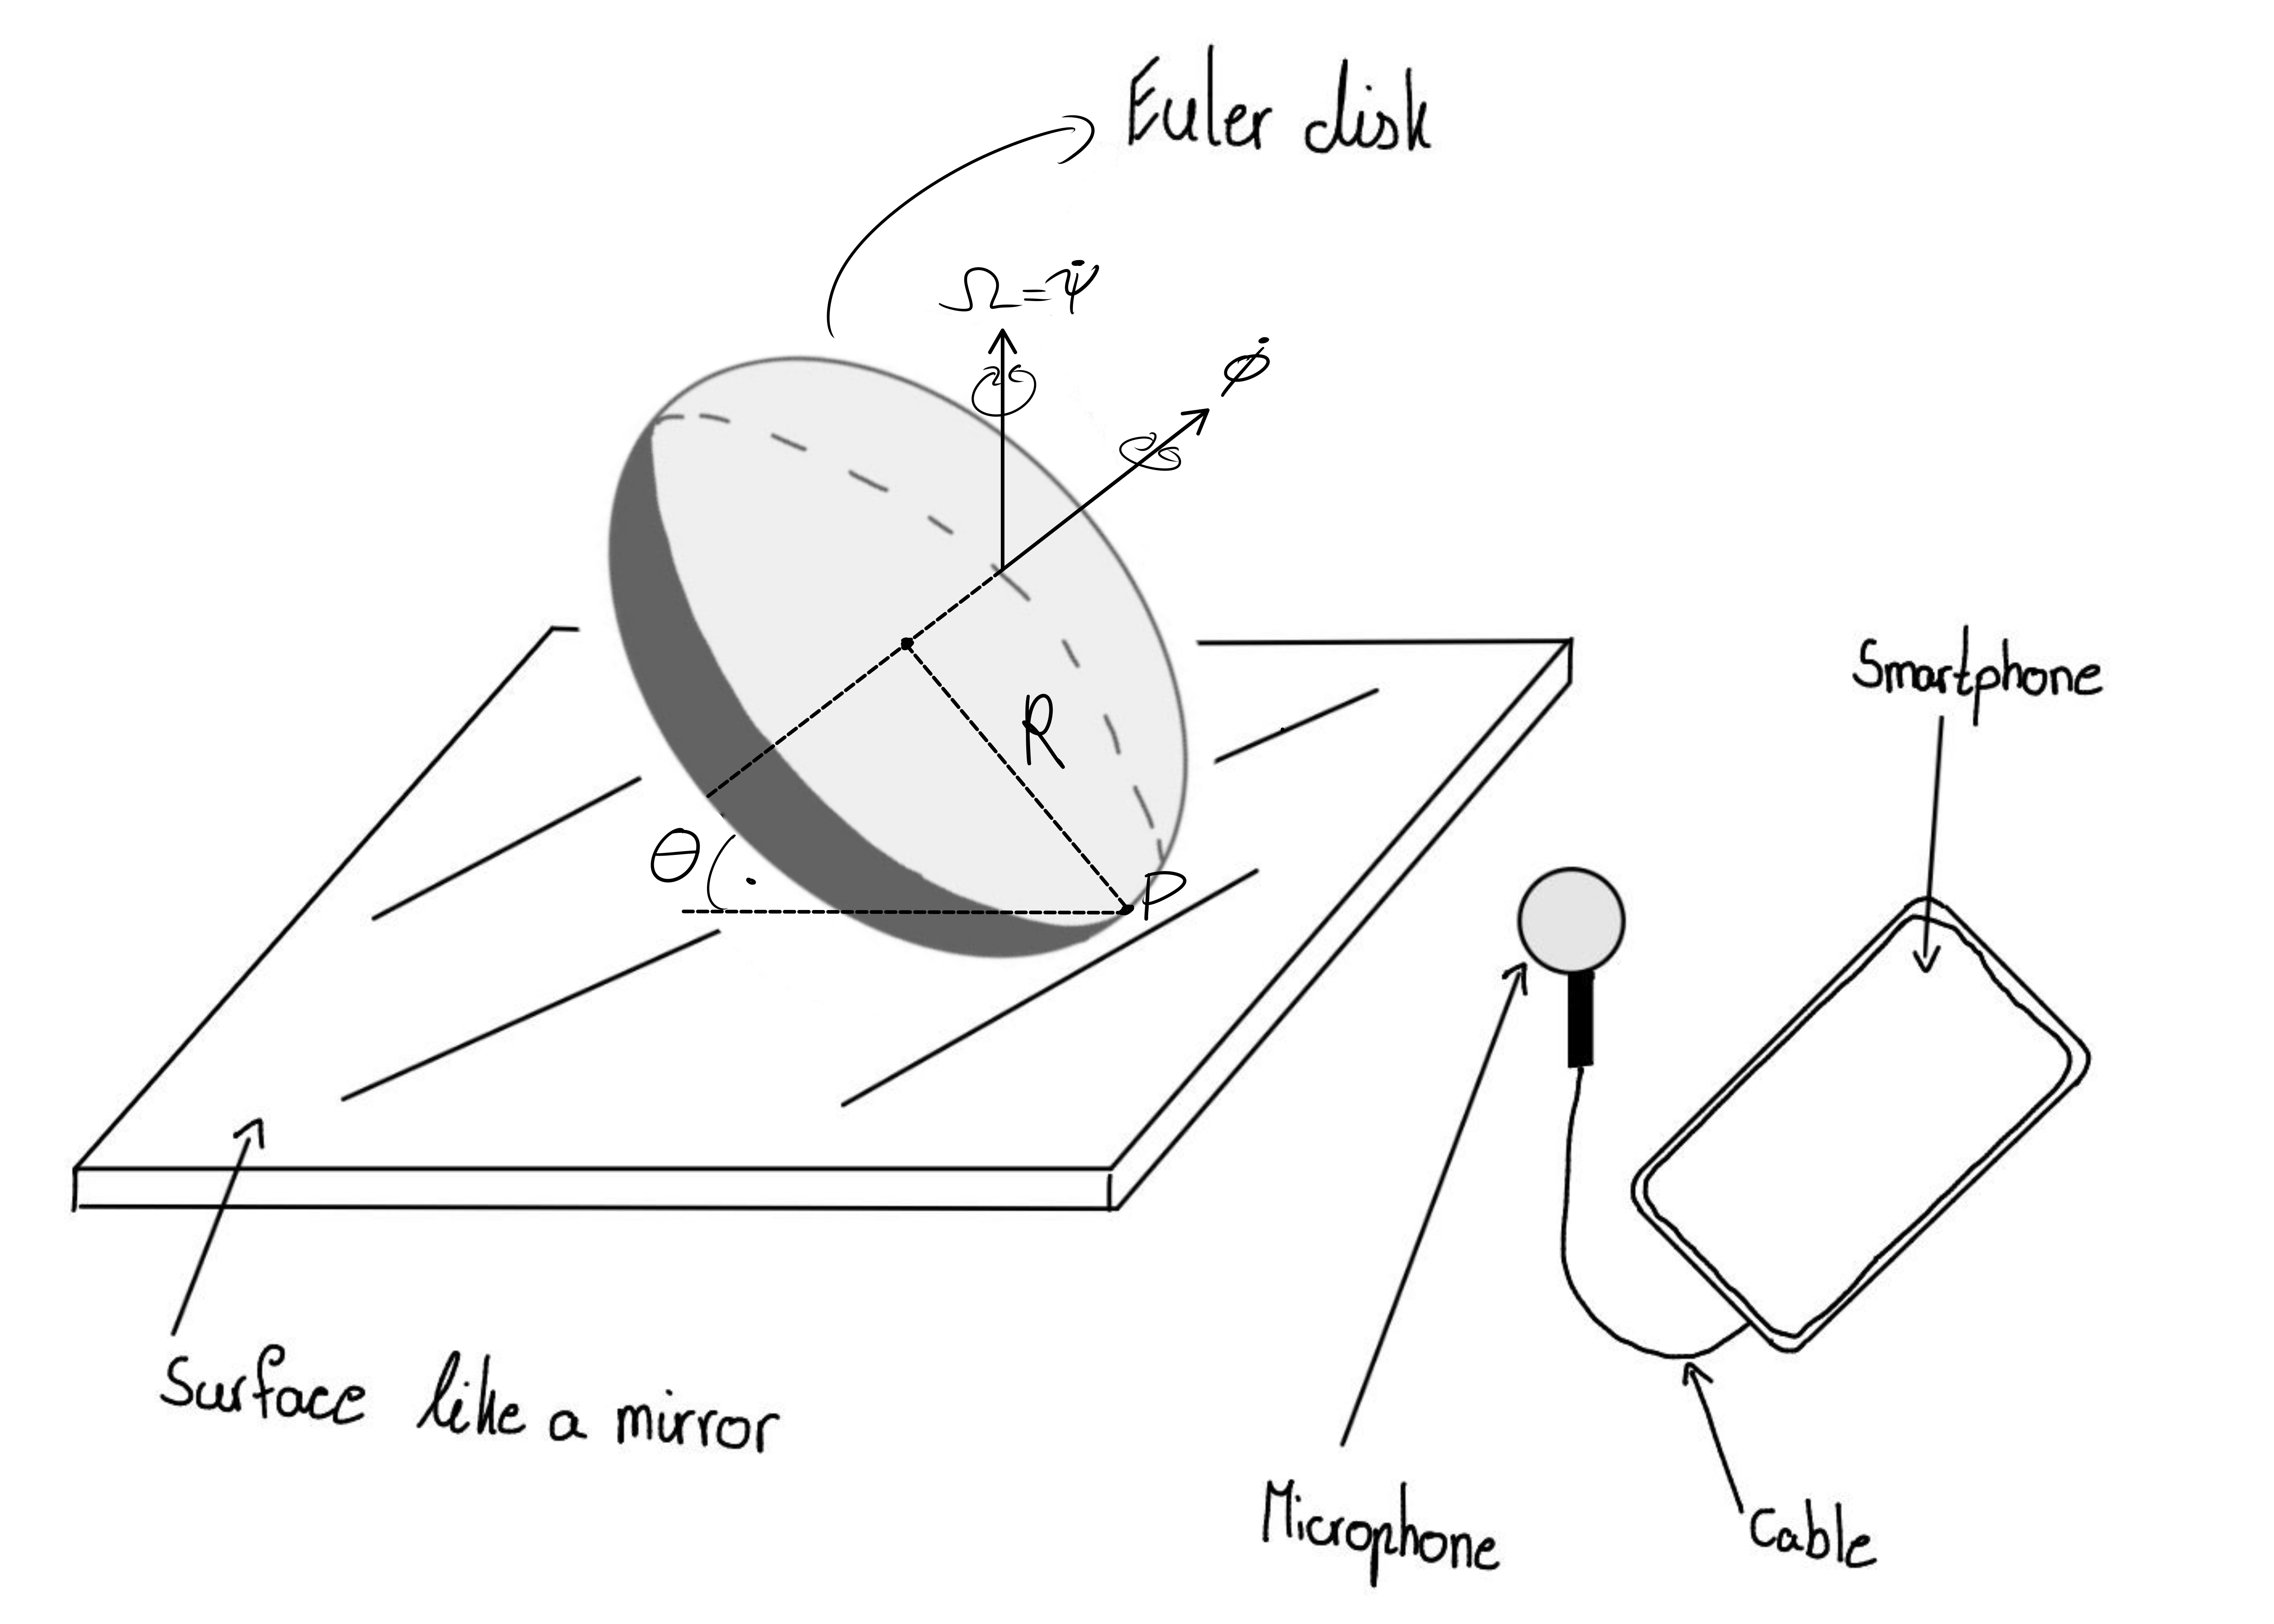
\includegraphics[width=1\textwidth]{euler_disc_sketch.png}
    \caption{Sketch of the experimental setup showing the Euler disk, the surface and the relevant quantities: the radius of the Euler disc $R$, the contact point between the disc and the surface $P$ ,the precession rate $\Omega=\dot{\psi}$, the spin rate $\dot{\phi}$, and the tilt angle $\theta$. Furthermore the measurement device, also the smartphone with a microphone is shown on the same sketch.}
    \label{fig:euler_disk_setup}
\end{figure}

The experimental setup consists of a rigid circular disk (Euler disk) spun on a flat horizontal surface. The disk of radius $R$ is inclined at an angle $\theta$ with respect to the surface and makes contact at a single point $P$, which moves around the center of mass with precession frequency $\Omega$. As the disk evolves in time, both the inclination angle and the precession rate change continuously.

The Euler disk will be spun manually on a horizontal surface while the emitted sound is recorded using a smartphone microphone placed at a close distance to the disk. Different surface materials  will be tested under otherwise identical conditions. All experiments will be performed in a quiet environment to minimize background noise. The recorded audio data will be transferred to a computer and analysed using Fourier-based spectral methods in order to extract the time-dependent dominant frequency $f(t)$. For each configuration, multiple measurements will be performed to ensure reproducibility.








\newpage
\section{rough ideas}
(measure with different surface)
((probably bad idea (???))measure with different disk)
(maybe different masses)
(coin)
[(bad idea) an Euler disk with a a small asymmetry (like a really small mass attached to one corner) ]
[DIFFERENCE OF EARLY AND LATE FIT WHICH ARE DETERMINED BY THE DOMINATING DISSIAPATION FORCE(ROLLING FRICTION FOR THE BEGİNNİNG AND THE AIR RESISTANCE FOR THE END)]
[video and sound recording and comparision with eachother]
[dependece on initial condition with stron, medium and weak launches of the disk]

Use $\chi^2$ to see which model is most precise.

\printbibliography

\end{document}
